\documentclass[10pt,a4paper,twocolumn]{article}
\usepackage[T1]{fontenc}
\usepackage[utf8]{inputenc}
\usepackage{lmodern}
\usepackage[a4paper,margin=20mm,columnsep=7mm]{geometry}
\usepackage{microtype}
\usepackage{amsmath,amssymb}
\usepackage{graphicx}
\usepackage{booktabs}
\usepackage{caption}
\usepackage{listings}
\usepackage{xcolor}
\usepackage[numbers,sort&compress]{natbib}
\usepackage{enumitem}
\usepackage[hidelinks]{hyperref}
\usepackage{url}

\captionsetup{font=small,labelfont=bf}
\setlist{nosep,leftmargin=*}
\graphicspath{{../results/}}

\lstdefinelanguage{Faust}{
  morekeywords={process,effect,with,import,library,declare,par,seq,sum,prod,route,ondemand,rdtable,waveform},
  sensitive=true,
  morecomment=[l]{//},
  morestring=[b]",
}
\lstset{
  language=Faust,
  basicstyle=\ttfamily\scriptsize,
  keywordstyle=\bfseries,
  commentstyle=\color{gray},
  columns=fullflexible,
  keepspaces=true,
  breaklines=true,
  frame=none,
  xleftmargin=0pt,
}

\newcommand{\faustrs}{faust-rs}
\newcommand{\probe}{\texttt{faustprobe}}
\newcommand{\coop}{\texttt{coopiano}}
\newcommand{\code}[1]{\texttt{#1}}

\title{From Prepared Notes to a Stream:\\Porting a Physically Modelled Piano from C++ to Faust,\\Checked Against the C++ Model Itself}
\author{St\'ephane Letz\\GRAME-CNCM, Lyon\\\texttt{letz@grame.fr}}
\date{October 2026}

\begin{document}
\maketitle

\begin{abstract}
\coop{} is a physically modelled piano written in C++17: a nonlinear felt hammer, unison strings with two polarizations, longitudinal phantom partials, action noises, dampers and a sustain pedal, a sympathetic string register, a modal soundboard imaged over four bridge regions and a feedback-delay room. It prepares each note offline, with a contact solve oversampled 32 times followed by a bank of decaying phasors. We port it to Faust as a stream, with the Rust Faust compiler \faustrs{}, and check the port against the C++ model itself: a small program includes its headers unchanged and writes the tables, the renders and the intermediate signals the comparisons need. Each string mode becomes a complex one-pole resonator driven with a first-order hold; the hammer is solved implicitly at the audio rate, with the felt's hysteresis rate taken at the same sample, which a one-sample lag would raise by 41\,\% in the fortissimo treble; a phantom partial is the product of two mode states. Over the keyboard the hammer's peak force is within 1.1\,\% of the C++ solve (an 11-sample contact excepted), the bridge force within 0.3\,dB, the sympathetic register identical to $10^{-12}$, and the whole instrument within 0.1\,dB of the C++ engine with the same stereo correlation. The soundboard is the C++ board's 732 modes with amplitudes fitted per bridge region: fitting the shared response and weighting it per region, the obvious shortcut, put the instrument 3.5 to 9.3\,dB off. The port also measured the compiler: function applications re-evaluated at every use, a normal form cubic in the length of a sum, and per-block coefficients that cost more than the strings; the paper says how the model is written around each, and what \faustrs{} should change.
\end{abstract}

\section{Introduction}

Porting a synthesizer between languages is usually checked by listening. A physically modelled piano makes that hard: two renders that differ by the random draws of a strike, the phase of a beating unison or the realization of a filtered noise do not sound identical even when both models are right, and two that sound alike may still disagree by a few decibels in a register nobody played. We take the opposite stance. The C++ model, \coop{}~\cite{coopiano}, is its own reference: a short program, \code{ref/dump.cpp}, includes its headers \code{piano.hpp} and \code{instrument.hpp} unchanged and writes everything the Faust model needs or should match: the fixed random tables, the per-key tuning draws, the post-contact excitation levels, the soundboard's modes and responses, single-note bridge forces, the force after the sympathetic register, and the stereo output of the full engine. The Faust model is then measured against these with \probe{}, the offline probe of \faustrs{}~\cite{faustrs}, which compiles a program, sets its controls, renders it and prints numbers.

The C++ model was not written for streaming. Each strike is \emph{prepared}: a 32-times oversampled integration of the hammer against every mode of every unison string, after which the modes are converted into decaying phasors, the phantom partials are added as further phasors, and the action noises are written into an attack buffer. A Faust program has no ``before the first sample'': it computes every signal at every sample. The port is therefore a reformulation, and this paper is about the reformulations that kept the C++ model's numbers (Sections~\ref{sec:voice}--\ref{sec:body}), the ones that did not and why (Section~\ref{sec:results}), and what the compiler made hard (Section~\ref{sec:compiler}).

\section{The C++ model}
\label{sec:model}

A key is described by about twenty register-dependent parameters (speaking length, tension, inharmonicity, strike position, decay times, hammer mass and felt law) interpolated over the note number, scaled by the thirty voicing controls of \code{default.ini}. Keys below MIDI~31 have one string, below 41 two, the others three, detuned by per-key draws.

\paragraph{Strings.} Each string is a sum of modes up to 17.5\,kHz, at most 600. A mode's frequency follows the stiff-string law, pulled by the reactive part of a random modal bridge admittance; its loss has a late-stage rate plus a frequency-dependent term. The hammer couples to a mode through the strike-point mode shape, softened by the felt's width; the bridge reads it through a weight carrying an empirical register-dependent voicing.

\paragraph{Hammer.} The felt law is $F = K\delta^p(1 + 0.12\,\dot\delta)$ for a compression $\delta > 0$, a power law with a Hunt--Crossley-like hysteresis~\cite{hunt1975,stulov1995}. \code{run\_contact} integrates the hammer and all modes by the symplectic Euler method at 32 times 44.1\,kHz until the hammer separates~\cite{chaigne1994}.

\paragraph{Free vibration.} At separation each mode's state is split into a vertical polarization, which carries most of the energy and decays fast (its rate follows the bridge admittance's real part, so modes near a board resonance drain sooner), and a horizontal one, slightly detuned and decaying at the late rate: the two-stage decay of real pianos~\cite{weinreich1977}. Both become phasors $z \mapsto z\,e^{(-\sigma + i\omega)/f_s}$; the damper blends each phasor's step toward a seated-damper rate over 40\,ms.

\paragraph{Phantom partials.} Longitudinal coupling is quadratic in the string slope, so pairs of modes drive the longitudinal string at their sum frequency~\cite{conklin1999,bank2005}. \code{add\_phantoms} forms, for neighbouring partials $i \le j \le i+3$ below 4.2\,kHz and keys below G\#3, the product of the two phasors, scaled, resonantly boosted near the longitudinal modes and bounded.

\paragraph{Body.} The engine sums the voices, adds the response of a sympathetic bank (88 keys, partials below 7\,kHz, open when a key is held, the pedal is down or the key has no damper; a key's own force is withheld from its own resonators), splits the force over four bridge regions and convolves it with the soundboard: 732 modes from 48\,Hz to 16.5\,kHz equalized by a minimum-phase filter that also removes three quarters of the narrow modal ripple, imaged per region for the first 0.2\,s and shared afterwards. A DC filter, an eight-line feedback delay network~\cite{jot1991}, an output gain and a soft limiter follow.

\section{The voice as a stream}
\label{sec:voice}

\subsection{Modes as complex one-poles}

A mode obeys $\ddot q + 2\sigma\dot q + (\omega^2+\sigma^2) q = g F(t)$. With the C++ convention $z = q - i(\dot q + \sigma q)/\omega$ (\code{polarization\_state}), $\mathrm{Re}\,z$ is the displacement and
\begin{equation}
\dot z = p\,z - i\frac{g}{\omega}F, \qquad p = -\sigma + i\omega.
\end{equation}
Over one sample $T$, with $F$ linear between $F_{n-1}$ and $F_n$ (a first-order hold),
\begin{equation}
z_n = \lambda z_{n-1} + G_0 F_{n-1} + G_1 F_n, \quad \lambda = e^{pT},
\end{equation}
with $G_1 = b\,T\varphi_2(pT)$, $G_0 = b\,T(\varphi_1 - \varphi_2)(pT)$, $b = -ig/\omega$, and the functions $\varphi_1(x) = (e^x - 1)/x$, $\varphi_2(x) = (e^x-1-x)/x^2$ of exponential integrators~\cite{hochbruck2010}, evaluated by their Taylor series near zero. The recursion is exact for a piecewise-linear force, so a mode's free decay is exactly the C++ phasor's.

The hammer needs the strike point's displacement \emph{before} the current force acts. Keeping $z_n$ as state would recompute it every sample; the voice keeps instead the free prediction $w_n = \lambda z_{n-1} + G_0 F_{n-1}$, which obeys
\begin{equation}
w_n = \lambda w_{n-1} + (\lambda G_1 + G_0) F_{n-1},
\end{equation}
so the strike point's free displacement, the bridge force and the phantoms all read $w$ directly; they differ from $z_n$ by $G_1F_n$, a fraction of one sample's motion, and only during contact. This change of state halved the voice's cost.

\paragraph{Polarizations.} The C++ splits the state at separation; splitting the \emph{drive} in the same proportions, into a vertical and a horizontal resonator, gives the same free vibration, since the modes are linear; during the few milliseconds of contact the two resonators decay at different rates, a difference the contact comparison of Section~\ref{sec:results} does not see.

\paragraph{Slots.} Faust needs the number of resonators at compile time. A voice has $N_S = 96$ slots shared by its strings, string by string: with $n_s$ strings, slot $k$ is partial $k \bmod (N_S/n_s) + 1$ of string $\lfloor k / (N_S/n_s)\rfloor$. A one-string bass key gets 96 partials, a trichord 32 per string. Every frequency, loss, decay share and bridge weight of \code{build\_string} and \code{collect\_phasors} is a function of the note and the voicing controls.

\subsection{The hammer, implicit at the audio rate}

At 44.1\,kHz the treble contact lasts a few dozen samples and the felt is stiff: for C8 at 20\,N we estimate the loop gain of an explicit scheme (the felt's tangent stiffness times the string's response over one sample) at about 6, far beyond what a force computed from the previous sample's compression can follow. The voice solves the delay-free loop~\cite{borin2000} instead. The strike point's displacement is $y_s = y_s^{\mathrm{free}} + R_s F_n$ and the hammer's $y_h = y_h^{\mathrm{free}} - R_h F_n$, where $R_s = \sum_k \bar a_k \mathrm{Re}\,G_{1,k}$ sums over the modes (readout $\bar a_k$ averaged over the unison, which receives equal shares of the force) and $R_h = T^2/6m_h$ for the same hold. The compression is $\delta = a - cF_n$ with $a = y_h^{\mathrm{free}} - y_s^{\mathrm{free}}$ and $c = R_h + R_s$. Its rate is linear in $F_n$ too, $\dot\delta = d_0 - d_1F_n$, from the free velocities and the direct velocity gains of the same modes. The felt law then gives, with $A = n_sK(1+0.12\,d_0)$ and $E = 0.12\,d_1 n_s K$,
\begin{equation}
\delta + c\,\frac{A\,\delta^p}{1 + E\,\delta^p} = a, \qquad F_n = \frac{A\,\delta^p}{1+E\,\delta^p},
\end{equation}
a scalar equation with a single root in $(0, a]$. Newton's method starts from the smaller of the two one-term solutions, $\min(a, (a/cA)^{1/p})$, which lies above the root, and five steps, kept in $[\delta/2, a]$, are enough.

Taking the rate $\dot\delta$ one sample late is tempting, since everything else is solved. It is not innocent. A numpy replica of both schemes on the C++ modes (\code{scripts/contact\_sim.py}), which reproduces the peak forces \probe{} measures on the Faust voice to 0.05\,\%, shows the lagged rate raising the fortissimo peak force by 41\,\% at C6 and 42\,\% at C7 while leaving the softer strikes within 1\,\% (Fig.~\ref{fig:contact}): the hysteresis term is largest at the start of a fast contact, where a one-sample lag is a large fraction of the compression time.

\begin{figure*}[t]
\centering
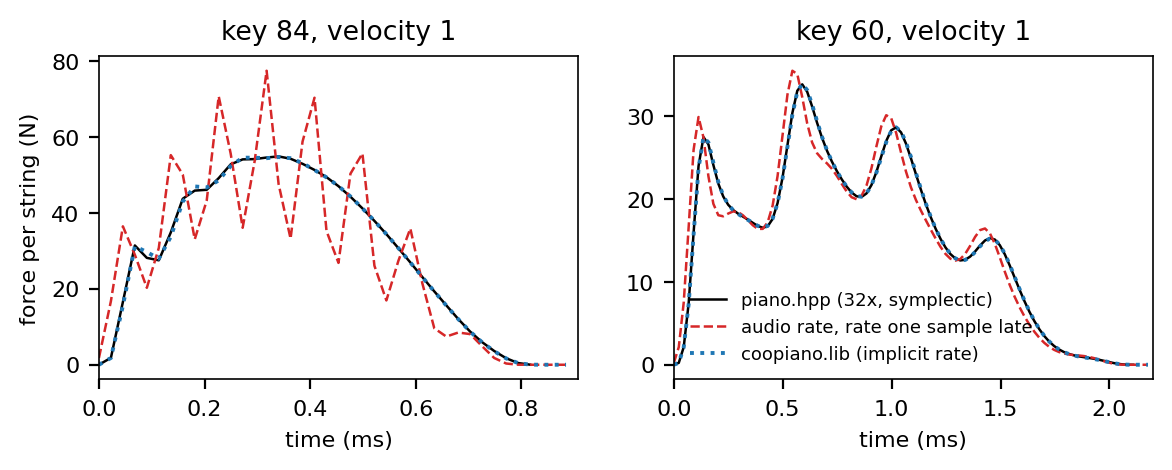
\includegraphics[width=\textwidth]{fig_contact.png}
\caption{Hammer force per string at velocity 1. Black: \code{run\_contact} (symplectic Euler at 32 times 44.1\,kHz). Red: the audio-rate implicit scheme with the felt's hysteresis rate taken one sample late. Blue: \code{coopiano.lib}, rate taken at the same sample.}
\label{fig:contact}
\end{figure*}

\subsection{Phantom partials as products}

A phantom phasor is the product of two parent phasors, so its frequency and decay are the sums of theirs. In a stream, the product of the two parents' current states \emph{is} that phasor, at no cost in state: released strings release their phantoms, and the damper's doubled rate on a phantom is the sum of its parents' rates. The voice forms the pairs of the same string and polarization at distances $d \le 2$ (the C++ allows 3; the next term is $0.55^3$, 15\,dB down), 288 pairs for 96 slots, each with a coefficient carrying the bridge voicing at the sum frequency and the longitudinal resonances. One identity matters for the compiler: the real part of $a\,b$ is written $(a_r - a_i)(b_r + b_i) + a_ib_r - a_rb_i$, because for $d = 0$ the textbook form contains $a_r^2$, which \faustrs{} normalizes to \code{pow(x, 2)}, a library call in its JIT: 391 of them per sample in the first version.

\subsection{What comes from tables}

Some quantities are random draws or the result of a solve the stream cannot redo. \code{ref/dump.cpp} writes them and \code{scripts/gen\_tables.py} turns them into \code{coopiano\_tables.lib}: the bridge admittance at 1\,Hz steps (a random modal sum), the per-key detuning draws, and \code{tone\_peak\_amp}, the excitation level after contact that scales every action noise, for 88 keys and 25 velocities (mean over four seeds). The action noises (keybed thump, structural knock, felt scrape, treble knock, damper felt) follow \code{prep\_note\_into}'s filters and envelopes on Faust noise.

One draw is per strike: each string's bridge readout is scaled by $1 + 0.13u$, $u$ uniform. The Faust voice samples it at the strike. Left to that, the first comparison showed every multi-string note 0.3 to 0.5\,dB louder than the C++: the C++ renders use seed~1, whose first draws are $-0.73$, $-0.73$, $-0.10$. A test-only entry point, \code{voice\_drawn}, takes the draws as arguments; with the seed's draws the offset vanished. A systematic offset can be a sample of one random draw.

\section{The body}
\label{sec:body}

\paragraph{Sympathetic register.} The bank is \code{SympatheticResonance} transcribed: 1002 resonator slots, a damped rotation per partial, the drive gated by the group's openness. A Faust effect sees only the summed force, not which keys are held, so two of the C++ behaviours need care. The withholding of a key's own force is linear: $\sum_k R_k(x - w\,x_k) = \sum_k R_k(x) - w\sum_k R_k(x_k)$, and the second term is computed by each voice from its own force, with the openness its key has in the shared bank, and handed to the body on a fifth channel. Driven by the C++ force of a C4 strike, the Faust bank and correction equal the C++ bank to $10^{-12}$ ($-248$\,dB). The opening of a key held silently is not modelled.

\paragraph{Soundboard.} The C++ board is a modal sum followed by an equalizer. The obvious port evaluates the equalizer at each mode's frequency and keeps the modes. It fails, with an error 1.3 times the response itself: the equalizer removes three quarters of the narrow ripple, so it is not smooth at the scale of a mode, and it is precisely at the modal peaks that it cuts. The port keeps the 732 poles and fits their complex amplitudes by least squares to the C++ response. The Gram matrix of damped exponentials has a closed form,
\begin{equation}
\sum_{n=0}^{N-1}\lambda_k^n\lambda_l^n = \frac{1 - (\lambda_k\lambda_l)^N}{1 - \lambda_k\lambda_l},
\end{equation}
and its conjugate counterpart, so no $67914 \times 1464$ matrix is formed; one Cholesky factorization serves every target. The shared response is fitted to $-25.5$\,dB.

The regions are where the port went wrong first. \code{make\_soundboard\_regions} weights each mode per region (a random smooth mode shape along the bridge and a constant-power pan) before the equalizer. Weighting the \emph{fitted} amplitudes in the same way seemed equivalent. It is not: neighbouring modes overlap, the least-squares amplitudes are not unique, and the fit's cancellations between neighbours do not survive a weighting. Fed the exact region forces of a C4 strike, that board was 3.5 to 9.3\,dB too loud in the engine's output, depending on the channel and the time window; on a region's response the magnitude error is visible across the spectrum (Fig.~\ref{fig:board}). Each region's response (head and shared tail, as the engine hears an impulse in that region) is now fitted on its own, for both channels: eight targets, one Gram matrix, $-22.8$ to $-25.7$\,dB. A mode is driven by the complex combination $\sum_r A_{r,k}x_r$ of the region forces, which costs as much as two real drives. The imaging is fixed at the C++ defaults (spread 0.7, position depth 0.5); a light body without imaging, one resonator per mode for both channels, is provided.

\begin{figure}[t]
\centering
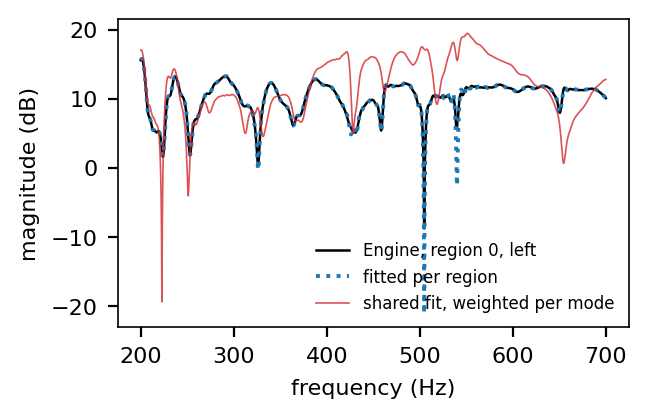
\includegraphics[width=\columnwidth]{fig_board.png}
\caption{Magnitude of region 0's left response (Engine), its per-region fit, and the shared fit weighted per mode as \code{make\_soundboard\_regions} weights the modes.}
\label{fig:board}
\end{figure}

\paragraph{Room and output.} \code{StereoReverb} is transcribed line by line: high-pass and predelay, six early taps, two diffusion all-passes per side, eight lines with an unnormalised Walsh--Hadamard feedback and one-pole damping. The DC filter, the gain and the soft limiter follow.

\section{Results}
\label{sec:results}

Table~\ref{tab:results} gathers the comparisons, all produced by \code{make results}; the figures come from the same renders.

\begin{table*}[t]
\centering
\small
\begin{tabular}{p{0.34\textwidth}p{0.6\textwidth}}
\toprule
Comparison & Result \\
\midrule
Hammer contact, 8 keys $\times$ 4 velocities, against \code{prep\_note} & peak force within 1.1\,\%; contact time within 1.3\,\% except at C8 (5 to 6\,\%, under one sample); C8 at velocity 1: $-14$\,\% peak force, an 11-sample contact \\
Bridge force, 12 notes from A0 to C8 (velocities 0.2 to 1), against \code{render\_bridge\_force} & level within 0.1\,dB in every window after 50\,ms, a release included (windows floored at $-100$\,dB of the peak), 0.3\,dB over the first 50\,ms; third-octave spectra within 0.6\,dB rms, except the attack of C3 forte (9.6\,dB rms over bands above 4\,kHz, see text) \\
Sympathetic register, driven by the C++ force & equal to $10^{-12}$ ($-248$\,dB) \\
Soundboard fit & shared response $-25.5$\,dB; regions $-22.8$ to $-25.7$\,dB; magnitude error 0.1\,dB median, under 0.7\,dB for 90\,\% of frequencies (50\,Hz--10\,kHz) \\
Whole instrument against \code{Engine}, C4, velocity 0.5, held 1\,s, dry and with reverb & level within 0.1\,dB per channel while the note sounds; left/right correlation 0.355 and 0.311 for both models; reverb tail within 0.1\,dB \\
\bottomrule
\end{tabular}
\caption{The Faust model against the C++ model (\code{results/*.txt}).}
\label{tab:results}
\end{table*}

\begin{figure*}[t]
\centering
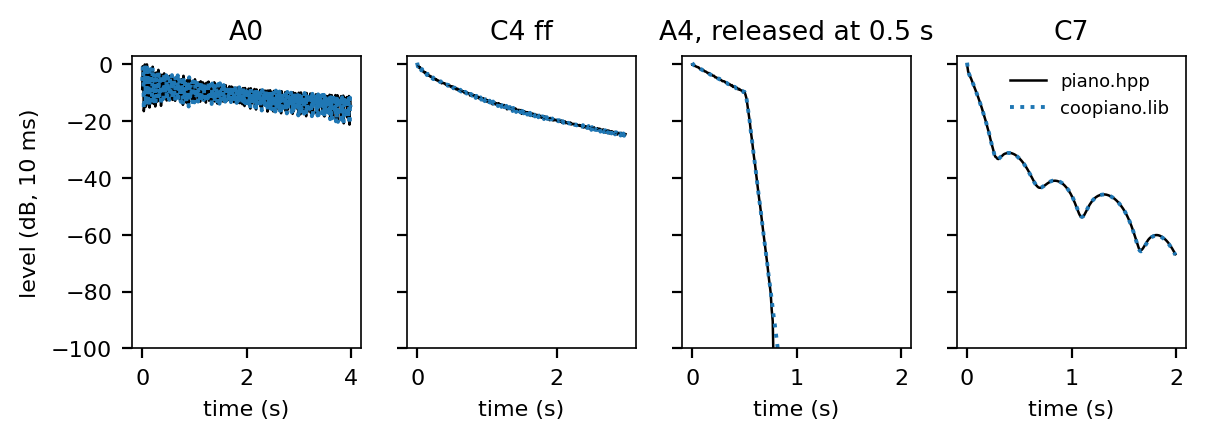
\includegraphics[width=\textwidth]{fig_notes.png}
\caption{Bridge force level (10\,ms windows) of four notes, \code{render\_bridge\_force} and the Faust voice with the seed's draws.}
\label{fig:notes}
\end{figure*}

\begin{figure*}[t]
\centering
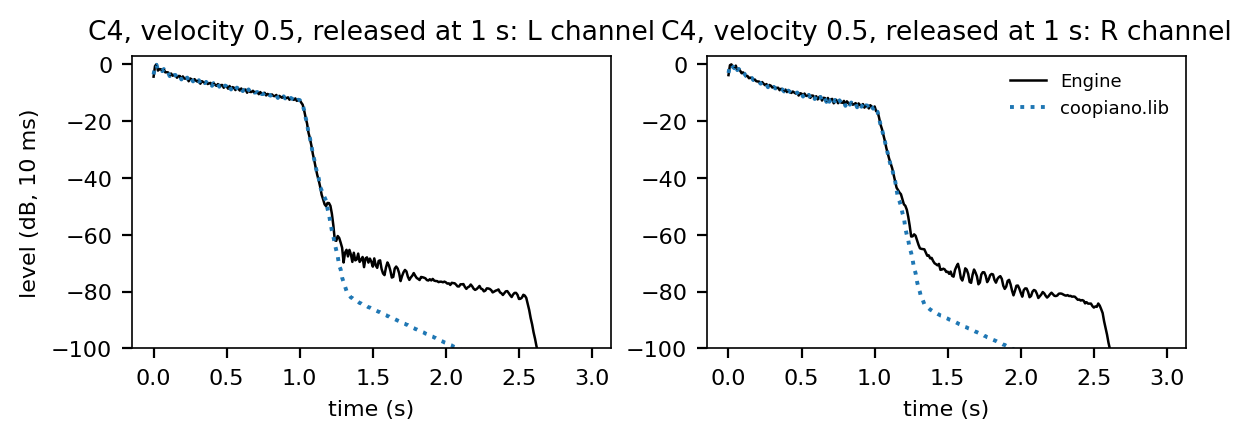
\includegraphics[width=\textwidth]{fig_engine.png}
\caption{The whole instrument: one strike through the sympathetic register, the imaged soundboard and the output stage, against coopiano's \code{Engine}.}
\label{fig:engine}
\end{figure*}

The contact, the notes (Fig.~\ref{fig:notes}) and the engine (Fig.~\ref{fig:engine}) agree where the models are the same model. The differences that remain have causes:
\begin{itemize}
\item \emph{Partials per string.} A trichord has 32 partials per string; C3 loses the C++ content above 4.5\,kHz, at most $-44$\,dB of the energy at the attack, which shows as the 9.6\,dB rms spectral difference over the bands above 4\,kHz. $N_S = 144$ gives 48 partials per string ($-67$\,dB) for 1.5 times the voice's cost.
\item \emph{The shortest contacts.} At C8 fortissimo the contact lasts 11 samples and the audio-rate scheme loses 14\,\% of peak force and 3\,\% of impulse.
\item \emph{Phantoms.} The per-pair amplitude bound of \code{bound\_phantom} and the $-80$\,dB pair threshold are not applied.
\item \emph{Release tails.} After a release, once the C++ engine is more than 60\,dB below the note, the Faust output is a further 15 to 25\,dB lower: the late tail of the board fit, where its error concentrates.
\item \emph{Noises.} Action noises are other realizations of the same filtered noise, and their level comes from the default voicing's contact solve.
\end{itemize}

\section{What the compiler made hard}
\label{sec:compiler}

The first complete voice did not compile in useful time: 435\,s, then a failure of the Cranelift JIT on a too large \code{compute} function. Each obstacle was measured and written around; together they are a report on \faustrs{}.

\paragraph{Evaluation does not memoize application.} The voice was first written as functions of the note, the slot and the polarization, called wherever a quantity was needed, many of them through lambdas (\code{force\_gains(\dots) : \textbackslash(g0r, \dots).(\dots)}). The generated code was right, each resonator once, thanks to hash-consing. But the evaluator caches a call by expression and environment \emph{identity}, and every application of a closure opens a new environment: a call inside a lambda body is re-evaluated at each application, and a chain of depth $D$ costs $2^D$. The voice took about 0.9\,s of evaluation per slot; even rewritten as dataflow (each slot a box evaluated once, publishing its signals on a bus that \code{route} distributes to the sums and the pairs) it still peaks at 17\,GB during evaluation, enough to make three concurrent compilations five times slower. The C++ compiler solved the same problem by memoizing \code{applyList} on the closure and its evaluated arguments; \faustrs{} has not ported it yet.

\paragraph{Long sums.} The normalization phase, \code{fir-prepare-normalize}, grows as the cube of a sum's length: at each partial sum of the left-nested chain \code{:>} builds, the search for a common factor tests every pair of terms, and \faustrs{} runs the simplification twice. The soundboard's two 732-term sums cost 16\,s, and 1.6\,s once summed in groups of 32 behind an opaque \code{max(x, -1e300)}.

\paragraph{Per-block coefficients.} Faust recomputes every control-rate expression at each block. For this voice that is 96 slots and 288 phantom coefficients: 11\,500 transcendental calls per block, about 180 per sample at 64-sample blocks, more than the strings. \faustrs{}'s \code{ondemand} runs a sub-program only on the samples where its clock fires. Clocked by ``the note or the voicing changed'', it would recompute the coefficients only then, except that the compiler hoists a computation depending only on controls out of the domain, back to block rate. Entering the note as a held audio-rate signal keeps it inside:
\begin{lstlisting}
on_change(chg, x, f) = (chg, ba.sAndH(chg, x)) : ondemand(f);
params = voice_params_on(chg, m);  // chg: note or voicing changed
\end{lstlisting}
The voice ran 1.8 to 2.7 times faster (bass and middle keys). The same mechanism lets the phantoms run only for keys below G\#3, and the sympathetic resonators of keys with dampers only while the dampers are lifted or for a second after; a sleeping key recomputes its parameters when it wakes, so a voicing change made while it sleeps is not lost.

\paragraph{Smaller traps.} \code{rad} and \code{fad} are reserved words (the differentiation primitives), which the C++ compiler accepts as identifiers, and the parse error does not say so; \code{-max(a, b)} does not parse, as in C++, with an obscure message; \code{A : f, B : g} reads as \code{A : (f, B) : g}, and the resulting arity error was reported on a shared \code{(\_, \_)} of an unrelated definition; \code{x*x} becomes \code{pow(x, 2)}, emitted as a library call where the C++ compiler emits a multiplication; \probe{}'s polyphonic mode panics when \code{effect} changes the channel count, so the instrument is checked by rendering the voice to a five-channel file that then drives the body; and \code{-vec} does not finish on the voice, its vector planning being quartic in the number of loops.

\paragraph{Cost.} Compiled by \faustrs{} to C++ and by clang at \code{-O3}, a sounding voice costs 2.9\,\% of an Apple M5 core. The imaged body costs 36\,\% of a core on the demo score without pedal and 45\,\% with it (the dampers' resonators then wake up); the light body 10\,\% and 22\,\% (\code{results/cost.txt}, best of three runs). The C++ engine convolves its board by partitioned FFTs; a modal board is the price of a model whose every sample is computed in Faust.

\section{Conclusion}

A model that prepares its notes can be ported to a stream without losing its numbers, if the port is checked against the model and not against an ear: the hammer, the strings and their two polarizations, the sympathetic register and the body agree with the C++ to a tenth of a decibel. The checks found the two errors that listening would have hidden: the hysteresis lag that inflates the fortissimo treble by 40\,\%, and the shortcut that moved the instrument's level by 5 to 9\,dB through the soundboard's regions. They also found a seed. On the compiler side, the port is a list of cases for \faustrs{}: an application memo in the evaluator, a normal form for long sums, and coefficients recomputed when their inputs change rather than at every block, which \code{ondemand} can express today with a held input.

\bibliographystyle{plainnat}
\bibliography{references}

\end{document}
